
In this chapter, we shall describe structure of the main input file and data formats of other input files.
In particular we briefly describe the GMSH file format used for both the computational mesh as well as for the input of general spatial data.


\section{Main Input File}
\label{sec:CONformat}

In this section, we shall describe structure of the main input file that is given either as the first positional argument or through 
the parameter \verb'-s' on the command line. First, we provide a quick introduction to the YAML file format. Then, we demonstrate the most important 
input structures on the examples. 







\subsection{YAML basics}
YAML is a human readable data format. It is designed to be both human readable and human editable. As it is not a markup languages, there are
no tags to determine type of the data. The indentation and justification is used instead for data organization. Moreover the used YAML format (version 1.2) is 
superset of the JSON format, another minimalist data serialization format where braces and brackets are used instead of indentation.
For the more detailed description see \href{https://en.wikipedia.org/wiki/YAML}{Wikipedia} 
for further technical details and for reference parsers for various programming languages see YAML \href{http://yaml.org/}{home page} .

\subsubsection{Hierarchy of Mappings and Lists}
Elementary data are organized to lists and mappings. Let us start with an example of a list:
\begin{verbatim}
# Example of list 
- 3.14                  # a number
- 2014-01-14            # a date
- Simple string.        # a string
- "3 is three"          # quoting necessary
- '3 is three'          # other qouting
- true                  # boolean
\end{verbatim}
Comments are started by a hash (\verb'#') which can appear anywhere on a line and marks the comment up to the end of line.
The the list follows with singel item per line preceded by a dash (\verb'-'). Any value starting by a digit is interpreted as a number
or date. Values starting with letter is interpreted as a string. Otherwise one may use double (\verb'""') or single (\verb"''") 
quotas to mark a string value explicitly. Finally some strings are interpreted as boolean values, it is recommended to use 
\verb'true' and \verb'false' (other possible pairs are e.g. \verb'yes/no', \verb'y/n', \verb'on/off'). 

Alternatively a list may be written in compact "JSON" way enclosing the list into brackets:
\begin{verbatim}
# Compact list
[ 3.14, 2014-01-14, Simple string.,
"3 is three", '3 is three'] 
\end{verbatim}

Other data structure is called mapping, which is also known as directory or associative array:
\begin{verbatim}
# Example of a mapping
pi: 3.14
date: 2014-01-14   
name: Mr. Simple String
\end{verbatim}

Again one may use also JSON syntax with mapping enclosed in braces:
\begin{verbatim}
# Compact mapping
{ pi: 3.14, date: 2014-01-14,   
name: Mr. Simple String }
\end{verbatim}

Mappings and lists may by mutually nested:
\begin{verbatim}
list:
    - one
    - two
    - 
        - three one 
        - three two
map:
    a: one 
    b: two
\end{verbatim}

A string may be split to more lines using {\it greater then} (\verb'>') and multi-line strings may be entered after {\it vertical line} (\verb'|'):
\begin{verbatim}
# single long string
one_line: >
    Single line string
    broken into two lines.
# multi line string
multi_line: |
    First line.
    Second line.
\end{verbatim}
In the first case the line breaks are replaced by space, in the second case the line breaks are preserved.
In both cases the leading indentation is removed.


\subsubsection{Tags}
YAML format defines a syntax for explicit specification of types of values including the types specific to an application.
The application specific tags are used by Flow123d to specify particular implementation of various algorithms or data types.
The general syntax of tags is quite complicated, so we present only the syntax used in the Flow123d input.
\begin{verbatim}
    field_a: !FieldFormula
        value: !!str "5 * x" 
    field_b:  !FieldFormula "5 * x"   
\end{verbatim}

The \verb'field_a' have specified evaluation algorithm \verb'FieldFormula', the key value have explicitly specified the default tag \verb'str'.
Note that default types are detected automatically and need not to be specified. On the third line we use even more compact way to 
express the same thing. Further details about usage of tags in Flow123d follows in Section \ref{sec:abstract}.

\subsubsection{References}
Anchors and references allows to reduce redundancy in the input data:
\begin{verbatim}
aux_name: &anchor_name John Smith
aux_man: &common_man
    sex: man
    city: Prague
    
people:
   - << *_common_man
     name: John Paul
   - << *_common_man
     name: *anchor_name
\end{verbatim}
On the first line, we define the anchor \verb'&anchor_name' for the value \verb'John Smith'. On the second line, 
we define the anchor \verb'&common_man' for the dictionary. Later, we use \verb'<<' to inject the dictionary 
referenced by \verb'*common_man'. Finally the anchor \verb'&anchor_name' is referenced by \verb'*anchor_name' to reuse the 
name \verb'John Smith'.

Ignoring the auxiliary keys \verb'aux_name' and \verb'aux_man' this is equivalent to:
\begin{verbatim}
people:
   - sex: man
     city: Prague
     name: John Paul
   - sex: man
     city: Prague
     name: John Smith
\end{verbatim}


\subsubsection{Gotchas}
\begin{itemize}
 \item Unquoted string values can not contain characters: colon \verb':', hash \verb'#', 
 brackets \verb'[]', braces \verb'{}', less then \verb'<', vertical bar \verb'|'.
 \item For indentation one can use only spaces tabs are not allowed. However, your editor editor may automatically convert tab to spaces.
 \item Boolean special strings must be quoted if you want to express a string. This is not problem for the Flow123d input.
 \item Numbers starting with digit zero are interpreted as octal numbers. 
\end{itemize}

\subsection{Flow123d specific constructs}
Flow123d have a subsystem for definition of the structure of the input file including preliminary checks for the 
correctness of the values. This subsystem works with elementary data types:
\begin{itemize}
 \item {\it Bool} corresponds to the YAML boolean values
 \item {\it Double}, {\it Integer} initialized from YAML numeric values. 
 \item {\it String}, {\it FileName}, {\it Selections} initialized from YAML strings.
\end{itemize}
Numerical values have defined valid ranges. FileName valus are used for reference to external files either for input or for output.
Selection type defines a finite number of valid string values which may appear on the input. 
These elementary types are further organized into Records and Arrays in order to specify strongly typed definition of the 
input data file. Array and Records forms so called input structure tree (IST).

In order to allow simple input of simple things while keeping complex things possible, the input system provides
so called automatic conversions from simple types to complex ones. 
So if the type of a value on input does not match the expected data type the automatic conversion tries to convert 
the given type to the expected type. Automatic conversion rules for individual composed types follows.

\subsubsection{Record $=$ Mapping}
A Record is initialized from the YAML mapping. However, in contrast to YAML mappings 
the Records have fixed keys with fixed types. 
This is natural as a Records is used for initialization of C++ objects which 
are also strongly typed. Every Record type have unique name and have defined list of its keys.
Keys are lowercase strings without spaces, possibly using digits and underscore. Every key have 
specified its type and default value specification. Default value specification can be:
\begin{description} 
 \item[obligatory] --- means no default value, which has to be specified at input. 
 \item[optional] --- means no default value, but value is needs not to be specified. Unspecified value usually means that you turn off some functionality.
 \item[default at declaration] --- the default value is explicitly given in declaration and is automatically provided by the input subsystem if needed
 \item[default at read time] --- the default value is provided at read time, usually from some other variable. In the documentation, 
 there is only textual description where the default value comes from.
\end{description}

Records that have all keys with default value or optional safe the single key $K$ may support autoconversion from an input of the type that match 
the type of the key $K$. For example:
\begin{verbatim}
  mesh: "mesh_file.msh"
\end{verbatim}
is converted to:
\begin{verbatim}
  mesh:
    mesh_file: "mesh_file.msh"
    regions: null
    partitioning: any_neighboring
    print_regions: false
    intersection_search: BIHsearch
\end{verbatim}
with the key \verb'regions' being optional and the last three keys having its default values. 


\subsubsection{Array $=$ List}
An Array is initialized from a YAML list. But, in opposition to the YAML mapping, the values in a single Array 
have all the same type. So the particular Array type is given by the type of its elements and a specification of its size range.

Automatic conversion performs kind of transposition of the data. It simplifies input of the list of records (or arrays) 
with redundant structure, e.g. consider input
\begin{verbatim}
  list:
    a: [1,2)
    b: 4
    c: [5,6]
\end{verbatim}
Assuming that key \verb'list' have the type Array of Records and keys \verb'a', \verb'b', \verb'c' are all numerical scalars this input is equivalent to
\begin{verbatim}
  list:
    - a: 1
      b: 4
      c: 5
    - a: 2
      b: 4
      c: 6
\end{verbatim}
The rule works as follows, if a key $K$ should have type Array, but some other type is on the input, 
we search through the input undeer the key $K$ for all Arrays $S$ standng instead of scalars.
All these arrays must have the same length $n$. Then the $i$-th element of the key $A$ array is
copy of the input keeping only $i$-th elements of the Arrays $S$.
As a special case if there are no Arrays $S$ a list with single element equal to the input is created.
Only this simplest conversion to an Array is applied if inappropriate type is found 
while the transposition is processed.





\subsubsection{Abstract (record)}
\label{sec:abstract}
An Abstract type allows a certain kind of polymorphism corresponding to a pure abstract class in C++ or to an interface in Java. 
Every Abstract type have unique name and set of Records that implements the Abstract. The particular type must be provided on input through the YAML tag.
See description of \hyperlink{sec:Fields}{Fields} below for examples.

An Abstract type may have specified the default implementation. If this default Record supports automatic conversion from one of its keys
we can see it as an automatic conversion from that key to the Abstract. For example
\begin{verbatim}
 conductivity: 2.0
\end{verbatim}
where conductivity is of Abstract type \verb'Field' with scalar values, is in fact converted to
\begin{verbatim}
 conductivity: !FieldConstant
    value: 2.0
\end{verbatim}
as the \verb'FieldConstant' is default implementation of the field and it is auto=convertible from the key \verb'value'. 





%\item[INCLUDE\_RECORD]:\\
%This is a simple inclusion of another file as a content of a record:
%\begin{verbatim}
%{
%        INCLUDE_RECORD = "<file name>"
%}
%\end{verbatim}
%
%\item[INCLUDE\_ARRAY]:\\
%\begin{verbatim}
%array=
%{
%        INCLUDE_ARRAY = "<file name>"
%        FORMAT = "<format string>"
%}       
%\end{verbatim}
%The reader will substitute the include record by a sequentially accessible array. The file has fixed number of 
%space separated data fields on every line. Every line becomes one element in the array of type record. Every line forms a 
%record with key names given by the \verb'<format string>' 
%and corresponding data taken form the line.

%The key difference compared to regular JSON arrays is that included arrays can be accessed only sequentially 
%within the program and thus we minimize reader memory overhead for large input data. The idea is to translate raw data into structured
%format and use uniform access to the data.

%Basic syntax for format string could be an array of strings --- formats of individual columns.
%Every format string is an address of key that is given the column. Onother possibility is to give an arbitrary 
%JSON file, where all values are numbers of columns where to take the value.

%[\dots better specify format string]


%Possible extensions:
% have sections in the file for setting time dependent data
% have number of lines at the beginning
% have variable format
% allow vectors in the 'line records']



\subsection{Input subsystem}
This section provides some implementation details about the Flow123d input subsystem. This may be helpful to better understand behavior of the program for 
some special input constructions.

\begin{figure}
 \begin{center}
 \includegraphics[scale=0.4]{\fig/input_subsystem.pdf}
 % input_subsystem.pdf: 0x0 pixel, -2147483648dpi, 0.00x0.00 cm, bb=
 \caption{Sturucture of the input subsystem. Grey boxes are not implemented yet.}
 \label{fig:input_subsystem}
 \end{center}
\end{figure}


\tbd{JAN BŘEZINA UPDATE}
The input subsystem of Flow123d is designed with the aim to provide uniform initialization of 
C++ classes and data structures. The scheme of the input is depicted on Figure \ref{fig:input_subsystem}.
The structure of the input is described by the Input Structure Tree (IST) of (usually static) objects which follows the structure of the classes.
The data from an input file are read by apropriate reader, their structure is checked against ITT and they are pushed into the Internal Storage Buffer (ISB).
An accessor object to the root data record is the result of the file reading. The data can be retrieved through accessors which combine 
raw data stored in in IBS with their meaning described in ITT. ITT can be printed out in various formats providing description of the input structure both for 
humans and other software.

Currently, the JSON input file format is only implemented and in fact it is slight extension of the JSON file format. On the other hand
the data for initialization of the C++ data structures are coded in particular way. Combination of this extension and restriction of the JSON file format produce 
what we call CON (C++ object notation) file format.


\section{Important Record Types of Flow123d Input}
Complete description of the input structure tree can be generated into HTML or LaTeX format. While the former one provides better interactivity 
through the hyperlinks the later one is part of this user manual. The generated documentation provides whole details for all keys, but 
it may be difficult to understand the concept of the input structures. This section is aimed to provide this higher level picture.


\subsection{Mesh Record}
\label{sec:Mesh}
The \hyperA{IT::Mesh}{mesh record} provides initialization of the computational mesh consisting of points, lines, triangles and tetrahedrons in the 3D ambient space.
Currently, we support only GMSH mesh file format \href{http://geuz.org/gmsh/doc/texinfo/gmsh.html#MSH-ASCII-file-format}{MSH ASCII}. 
The input file is provided by the key \hyperA{Mesh::mesh-file}{{\tt mesh\_file}}. The file format allows to group elements into {\it regions} 
identified by a unique label (or by ID number). The regions with labels starting with the dot character are treated as {\it boundary regions}. 
Their elements are removed from the computational domain, however they can be used to specify boundary
conditions. Other regions are called {\it bulk regions}. Every element lies directly in just one {\it simple region} while the simple regions may be 
grouped into composed regions called also region sets. A simple region may be part of any number of composed regions.
Initial assignment of the simple regions to the elements is given by the physical groups of the input GMSH file. Further
modification of this assignment as well as creation of new simple or composed regions can be done 
through the list of operations under the key \hyperA{Mesh::regions}{{\tt regions}}. The operations are performed in the order given by the input.
Operation \hyperA{Region::From-Id}{{\tt From\_Id}} sets the name of a simple region having only ID in the input GMSH file. Operation 
\hyperA{Region::From-Label}{{\tt From\_Label}} can rename a simple region. Operation \hyperA{Region::From-Elements}{{\tt From\_Elements}}
assign new simple region to the given list of elements overwriting their region given by the input mesh file. Finally operations 
\hyperA{Region::Union}{{\tt Union}}, \hyperA{Region::Difference}{{\tt Difference}} and \hyperA{Region::Intersection}{{\tt Intersection}}
implements standard set operations with both simple and complex regions resulting in new composed regions.




\subsection{Input Fields}
Input of every equation contains the key \verb'input_fields' used consistently for the input of the equation parameters 
in form of general time--space dependent fields.  The input fields are organized into a list of {\it field descriptors}, see 
e.g. \hyperA{IT::Flow-Darcy-MH-Data}{\tt Data} record, the field descriptor of the DarcyFlow equation.
The field descriptor is a Record with keys 
\hyperA{Flow-Darcy-MH-Data::time}{{\tt time}}, 
\hyperA{Flow-Darcy-MH-Data::region}{{\tt region}}, 
\hyperA{Flow-Darcy-MH-Data::rid}{{\tt rid}}
and further keys corresponding to the 
names of input fields supported by the equation. The field descriptor is used to prescribe
a change of one or more fields in particular time (key \verb'time') and on particular region given  by the name (key \verb'region', preferred way) 
or by the region id (key \verb'rid'). 
The array is processed sequentially and latter values overwrite the previous ones. Change times of a single field must form a non-decreasing sequence.
Changes in fields given by the fields descriptor are interpreted as discontinuous changes of the changed fields
and equations try to adopt its time stepping to match these time points. This is in contrast with changes of the field values given by
the evaluation algorithms, these are always assumed to be continuous and the time steps are not adapted. 



Example:
\begin{verbatim}
input_fields = [   
    { // time=0.0  - default value
        r_set="BULK",
        conductivity=1   // setting the conductivity field on all regions
    },
    {
        region="2d_part",
        conductivity=2  // overwriting the previous value
    },
    {   time=1.0,
        region="2d_part",
        conductivity={
            // from time=1.0 we switch to the linear function in time
            TYPE=FieldFormula,
            value="2+t"      
        }    
    },
    {   time=2.0,
        region="2d_part",
        conductivity={
            // from time=2.0 we switch to elementwise field, but only
            // on the region "2d_part"
            TYPE=FieldElementwise,
            gmsh_file="./input/data.msh",
            field_name="conductivity"
        }
    }    
]               
\end{verbatim}



\subsubsection{Field Algorithms}
\label{sec:Fields}
A general time and space dependent, scalar, vector, or  tensor valued function can be specified through the family of abstract records 
\verb'Field:R3 -> X', where $X$ is a type of value returned by the field, which can be:
\begin{itemize}
 \item $T$ --- scalar valued field, with scalars of type $T$
 \item $T[d]$ --- vector valued field, with vector of fixed size $d$ and elements of type $T$
 \item $T[d, d]$ --- tensor valued field, with square tensor of fixed size and elements of type $T$
\end{itemize}
the scalar type $T$ can be one of
\begin{itemize}
 \item {\bf Real} --- scalar real valued field
 \item {\bf Int}  --- scalar integer valued field
 \item {\bf Enum} --- scalar non negative integer valued field. Values on the input are of the type Selection.
\end{itemize}

Each of these abstract records have the same set of descendants which implement various evaluation algorithms of the fields. These are
\begin{description}
 \item[FieldConstant] --- field that is constant both in space and time
 \item[TimeFunction] --- field that is constant in space and continuous in time. Values are interpolated (currently only linear interpolation) from 
 the sequence of time-value pairs provided on input.
 \item[FieldFormula] --- field that is given by runtime parsed formula using $x,y,z,t$ coordinates. The \href{http://warp.povusers.org/FunctionParser/}{Function Parser} library is used
 with syntax rules described \href{http://warp.povusers.org/FunctionParser/fparser.html#literals}{here}.
 \item[FieldPython] --- field can be implemented by Python script either specified by string (key \hyperA{FieldPython::script-string}{{\tt script\_string}}) 
 or in external file (key \hyperA{FieldPython::script-file}{{\tt script\_file}}. 
 \item[FieldElementwise] --- discrete field, currently only piecewise constant field on elements is supported, the field can given by 
 the \href{http://geuz.org/gmsh/doc/texinfo/gmsh.html#MSH-ASCII-file-format}{MSH ASCII} file specified in key \hyperA{FieldElementwise::gmsh-file}{{\tt gmsh\_file}} and field name in the file given 
 by key \hyperA{FieldElementwise::field-name}{{\tt field\_name}}. The file must contain same mesh as is used for computation.
 \item[FieldInterpolated] --- allows interpolation between different meshes. Not yet fully supported.
\end{description}

Several automatic conversions are implemented. Scalar values can be used to set constant vectors or tensors. Vector value of size $d$ can be used to set diagonal tensor $d\times d$.
Vector value of size $d(d-1)/2$, e.g. $6$ for $d=3$, can be used to set symmetric tensor. These rules apply only for FieldConstant and FieldFormula.
Moreover, all Field abstract types have default value \verb'TYPE=FieldConstant'. Thus you can just use the constant value instead of the whole record.

Examples:
\begin{verbatim}
input fields:
   - conductivity: 1.0
     # is equivalent to
   - conductivity: !FieldConstant
        value=1.0
   
   - anisotropy: [1 ,2, 3] # diagonal tensor
     # is equivalent to
   - anisotropy: !FieldConstant
        value=[[1,0,0],[0,2,0],[0,0,3]]

     # concentration for 2 components   
   - conc: !FieldFormula  ["x+y", "x+z"]
     # is equivalent to
   - conc: 
       - !FieldFormula
         value: "x+y"
       - !FieldFormula
         value: "x+z"
\end{verbatim}

\subsubsection{Field Units}
Every field (e.g. conductivity or storativity) have specified unit in terms of powers of the base SI units. 
The user, however, may set input in different units specified by the key \verb'unit' 
supported by every field algorithm. The key have type \verb'Unit' record with a single auto convertible key 
\verb'unit_formula'. The unit formula is evaluated  into a coefficient and an SI unit. The resulting SI unit 
must match expected SI unit of the field, while the input value 
of the field (including values from external files or returned by Python functions)  
is multiplied by the coefficient before further processing.

The unit formula have form: {\tt <UnitExpr>;<Variable>=<Number>*<UnitExpr>;...,}
where {\tt <Variable>} is a variable name and {\tt <UnitExpr>} is a units expression
which consists of products and divisions of terms, where a term has form \verb'<Base>^<N>', 
where {\tt <N>} is an integer exponent and {\tt <Base>} is either a base SI unit, 
a derived unit, or a variable defined in the same unit formula.
Example, unit for the pressure head: 
\begin{verbatim}
   MPa/rho/g_; rho = 990*kg*m^-3; g_ = 9.8*m*s^-2
\end{verbatim}


\subsection{Output Records}
\tbd{JAN BŘEZINA:OUTPUT RECORDS}
